\section{Introduction}

Il s'agit dans ce chapitre d'introduire les probl\'ematiques et m\'ethodologies qui nous guideront dans notre \'etude de l'utilisation de l'asservissement visuel pour les robots parall\`eles \`a c\^ables. Notre objectif est double: il s'agit dans un premier temps d'ajouter des fonctionnalit\'es de saisie et manipulation d'objets \`a nos prototypes existants, et d'am\'eliorer les propri\'et\'es de ces m\^emes prototypes dans un second temps.

Pour cela, nous  \'evoquons dans une premi\`ere section les avantages et inconv\'enients des structures parall\`eles comparativement aux structures en s\'erie. Les sp\'ecificit\'es des manipulateurs \`a c\^ables sont introduites dans une deuxi\`eme section, suivie par un rappel des mod\`eles g\'eom\'etriques et cin\'ematiques des manipulateurs parall\`eles \`a c\^ables. Nous pr\'esentons dans la section suivante le prototype sur lequel nos exp\'erimentations et validations ont \'et\'e effectu\'ees, avant d'introduire quelques notions fondamentales pour la suite.

Apr\`es un rappel des mod\`eles d'asservissement visuel, nous introduirons les sp\'ecificit\'es de notre choix de configuration, dont nous montrerons de quelle mani\`ere il se d\'emarque des travaux existants dans ce domaine pr\'ecis. Nous pourrons alors conclure par l'exposition des probl\'ematiques \`a partir desquelles nous nous sommes propos\'e de mener cette \'etude, ainsi que des choix m\'ethodologiques qui en auront guid\'ee la r\'ealisation.

\subsection{Manipulateurs s\'erie et parall\`eles}

C'est incontestablement l'industrie qui aura \'et\'e le principal vecteur de d\'eveloppement de la robotique ces deux derniers si\`ecles. L'introduction des robots dans les usines s'inscrit dans une d\'emarche d'augmentation de la productivit\'e et d'am\'elioration de la manufacture. Cela aura permis d\`es lors de soulager le travailleur humain dans des situations de travail p\'enible et/ou r\'ep\'etitif, et d'augmenter ses comp\'etences en permettant par exemple une pr\'ecision qu'il ne saurait fournir seul, ou la possibilit\'e de d\'eplacer des charges \'elev\'ees. Si la grande diversit\'e que recouvre aujourd'hui le terme de {\it robot} rend extr\^ement difficile l'\'elaboration d'une d\'efinition g\'en\'erique, nous pouvons cependant en d\'eriver des sous-cat\'egories plus faciles \`a appr\'ehender. Parmi celles-ci, nous distinguons en particulier la classe des manipulateurs dont l'objectif sera le d\'eplacement d\'objets dans l'espace. Un manipulateur sera constitu\'e de mani\`ere g\'en\'erale d'une base et d\'un organe terminal, reli\'es par une ou plusieurs cha\^ines cin\'ematiques plus ou moins \'elabor\'ees.

Une cha\^ine cin\'ematique est caract\'eris\'ee par une succession de solides reli\'es par des articulations. Les articulations simples peuvent \^etre de nature {\it prismatique} \ref{intro:fig0view0} -- permettant la translation d'un solide par rapport \`a l'autre -- ou {\it roto\"ides} \ref{intro:fig0view1} -- effectuant un mouvement de rotation autour d'un axe donn\'e. Des articulations complexes sont obtenues \`a partir de la combinaison de mouvements prismatiques et roto\"ides : une articulation cylindrique \ref{intro:fig0view2} permet par exemple la combinaison d'un mouvement de translation selon un axe donn\'e et d'un mouvement de rotation autour de ce m\^eme axe ; une articulation sph\'erique \ref{intro:fig0view3} combinera trois rotations).

\begin{figure}[!h]
  \centering
      \subfloat[Articulation simple de type prismatique]{\label{intro:fig0view0}
    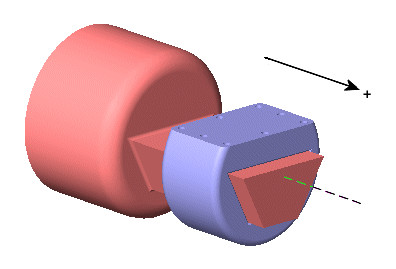
\includegraphics[width=.22\linewidth]{./intro/figures/prismaticJoint.jpg}} \hfill
    \subfloat[Articulation simple de type roto\"ide]{\label{intro:fig0view1}
    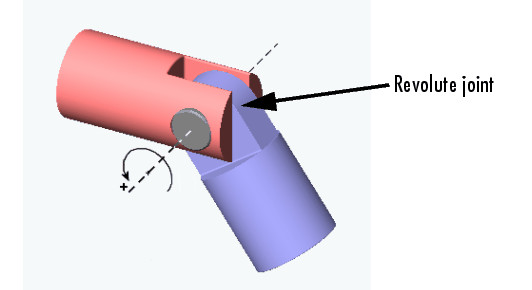
\includegraphics[width=.22\linewidth]{./intro/figures/revoluteJoint.jpg}} \hfill
  \subfloat[Articulation compos\'ee de type cylindrique]{\label{intro:fig0view2}
    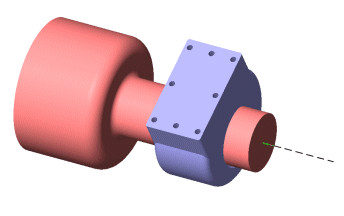
\includegraphics[width=.22\linewidth]{./intro/figures/cylindricalJoint.jpg}} \hfill
  \subfloat[Articulation compos\'ee de type sph\'erique]{\label{intro:fig0view3}
    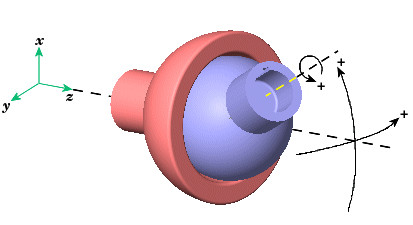
\includegraphics[width=.22\linewidth]{./intro/figures/sphericalJoint.jpg}}
    \caption{\footnotesize{Diff\'erents exemples d'articulations.}}
\label{intro:fig0}
\end{figure}

